\documentclass{article}
\usepackage[utf8]{inputenc}
\usepackage{graphicx}
\usepackage{geometry}
\usepackage{amsmath}
\usepackage{amsfonts}
\usepackage{float}
\usepackage{caption}
\usepackage{subcaption}
\usepackage{enumitem}

\geometry{left=25mm, top=25mm, right=25mm, bottom=25mm}

\title{PHY407 Lab 8}
\author{Pierino Zindel (1002429703) and Hayden Johnson (1002103537)}
\date{November 2, 2018}

\begin{document}

\maketitle

\noindent \textbf{Distribution of work:} Question 1 was completed by Pierino. Question 2 was completed by Hayden.

\section{Temperature Distribution in a Heat Conductor}

\subsection{Part b)}

We seek to evaluate the impact of overrelaxation by examining the solution to the heat equation with the given boundary conditions after 100 iterations using the Gauss-Seidel method with both regular relaxation ($w=0$) and overrelaxation with $w=0.9$. 

We did this by making the simple modification to our code from part a) to run the loop which computes new values of the temperature iteratively only 100 times, instead of until a target precision was reached. A plot of the temperature after 100 iterations with $w=0.0$, which corresponds to regular relaxation, is shown in figure \ref{fig:1b_w=0.0}, while a plot of the temperature of 100 iterations with $w=0.9$, which is an example of overrelaxation, is shown in figure \ref{fig:1b_w=0.9}. 

\begin{figure}[H]
	\centering
	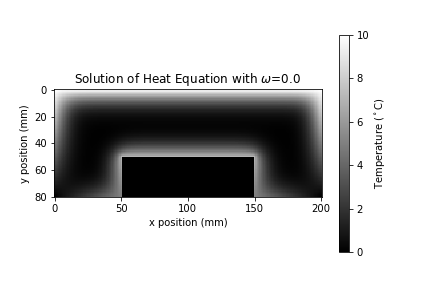
\includegraphics[width=0.8\textwidth]{../images/q1_b_0p0.png}
	\caption{Plot of temperature distribution after 100 iterations using Gauss-Seidel method, with regular relaxation ($w=0.0$).}
	\label{fig:1b_w=0.0}
\end{figure}

The two solutions are qualitatively quite different; in the case of regular relaxation (figure \ref{fig:1b_w=0.0}), the initial value of $T\approx 0$ still persists throughout much of the interior of the domain after 100 iterations, and we can see that the heat from the non-zero boundaries is beginning to permeate gradually through towards the interior of the domain, but it has not gotten very far. The drop off from the non-zero boundaries moving in towards the interior is thus quite steep.

Contrast this with the case of overrelaxation (figure \ref{fig:1b_w=0.9}), where the solution after the same number of iterations (100) looks quite smooth throughout the whole of the domain, and we can see that the heat from the boundaries has penetrated all the way through to the center of the domain. Thus, we can conclude that the overrelaxation Gauss-Seidel method has gotten far closer to the steady-state solution than regular relaxation Gauss-Seidel method has in the same number of iterations, and thus that the overrelaxation method should also converge to the steady-state solution more quickly than the regular relaxation method. Given what we know about how overrelaxation tries to accelerate the convergence by ``overestimating" the correction at each iteration, this makes perfect sense.


\begin{figure}[H]
	\centering
	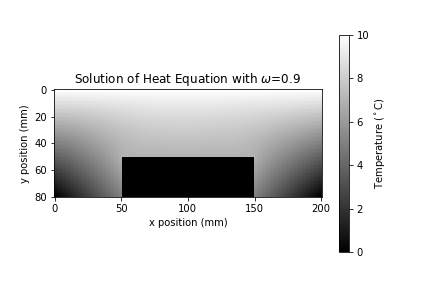
\includegraphics[width=0.8\textwidth]{../images/q1_b_0p9.png}
	\caption{Plot of temperature distribution after 100 iterations using Gauss-Seidel method, with overrelaxation ($w=0.9$).}
	\label{fig:1b_w=0.9}
\end{figure}

\subsection{Part c)}

We seek to calculate the steady-state temperature at each grid point to a precision of $10^{-6}$ $^\circ C$, using overrelaxation Gauss-Seidel with $w=0.9$, and also animate the process of iteratively solving the equation.

We adapted our program from part a) to use the Gauss-Seidel overrelaxation method with $w=0.9$ to iteratively solve the heat equation on the specified domain with the given boundary conditions, and to proceed until the maximum change in value between one iteration and the next at any single point in the domain was less than the specified target precision of $10^{-6}$ $^\circ C$. Doing this, we found the converged solution plotted in figure \ref{fig:1c}. Notice that this looks quite similar to the solution found after 100 iterations using the overrelaxation method in part b) (figure \ref{fig:1b_w=0.9}), indicating that the answer was already quite close after only that many iterations.

From the animation, it was clear that, before the solution got close to converging, the values of the temperature in the array were not symmetric about the line $x=10$, even though the domain and boundary conditions being symmetric about this line imply that the final solution should be too (as indeed it is). This temporary asymmetry is consequence of the way in which the Gauss-Seidel method updates the temperature values, moving in this case from left to right and top to bottom, and at each step using the most recent value available. This means that when the new value at each point is computed, it uses values from the current iteration from its neighbours above and to the left of it, while it uses values from the old iteration from its neighbours below and to the right of it. Hence, information initially can propagate much more quickly downwards and to the right than it does in the opposite directions - in theory, a large value at the top left of the grid could see its influence spread all the way to the bottom right in the course of a single iteration, whereas information can propagate from right to left and from bottom to top at a maximum speed of a single grid square per iteration. Eventually, as we get nearer and nearer to the converged solution, the small differences between the current values and the equilibrium values mean that there are no longer any large discrepancies to be propagated, and this asymmetry ceases to matter, yielding our (approximately) correct converged solution.

Using the coordinate system as it is defined by the axes in figure \ref{fig:1c}, the value of the converged solution at $x=2.5$cm, $y=1.0$cm is $T = 9.030218 ^\circ$C.

\begin{figure}[H]
	\centering
	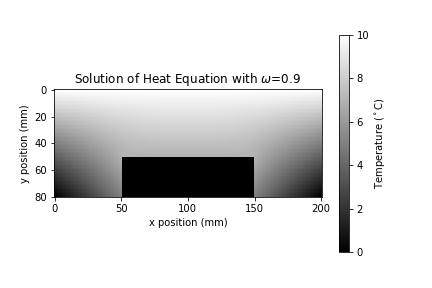
\includegraphics[width=0.8\textwidth]{../images/q1_c.png}
	\caption{Plot of temperature distribution created using Gauss-Seidel method, with overrelaxation ($w=0.9$), with a target precision of $1.0\times 10^{-6}$.}
	\label{fig:1c}
\end{figure}


\end{document}